\section{Introduction}\label{sec:intro}

% batching is important
Transaction processing is a fundamental aspect of database functionality, and improving OLTP system performance has long been a key research goal in our community. It is well-known that the throughput of OLTP systems can be increased through \emph{batching}-based optimizations, whereby some component buffers a number of transactions or requests as they arrive and processes them as a group.

% batching for obvious reason: low level
Batching can improve system performance for several reasons. First, it increases the efficiency of communication by packing messages~\cite{ding2015centiman,friedman1997packing}. Second, it amortizes the cost of system calls by condensing multiple requests into a single one, as in group commit~\cite{debrabant2013anti,hagmann1987reimplementing}. Third, it reduces the number of requests by discarding duplicate or stale requests, such as writes to the same record~\cite{faleiro2014lazy}. However, all of those are local optimizations based on low-level techniques.

% our proposal at a high level: batching at higher level for OCC 
We propose an OLTP system design that embraces batching as a core design
principle throughout transaction execution.  In particular, we explore the
benefits of incorporating reordering into batching in optimistic concurrency control (OCC) to reduce conflicts~\cite{kung81tods}. OCC is a popular concurrency control protocol due to its low overhead in low-contention
settings~\cite{adya97podc, baker11cidr, bernstein2015optimizing,bernstein11cidr,
bernstein11vldb, corbett12osdi,warp, patterson12vldb,peng10osdi}. However, it
wastes resources when conflicts are frequent~\cite{agrawal1987concurrency}. We
show batching and reordering reduce the number of conflicts, improve
throughput and latency, and allow us to use OCC with higher-contention workloads.


Figure~\ref{fig:occ_arch} shows a loosely coupled OCC-based transaction processing system with centralized validation. The system consists of three components: processors, storage nodes, and a single validator. External clients issue transactions to the system. On arrival into the system, each transaction is assigned to a processor and enters its \emph{read} phase. The processor sends read requests to the storage, executes the transaction, and performs writes to a local workspace. After it has processed the transaction, it sends information about the transaction's reads and writes to the validator. 

The transaction now enters the \emph{validation} phase. In OCC with \emph{backward validation}, the validator checks if a particular transaction conflicts with any previously committed ones. \eat{, and makes a``success'' or ``failure'' validation decision.}
%jg01: We need a citation after ``decision.''
One example of a conflict that would fail validation is a \emph{stale read}. Suppose a transaction $t$ reads an object $x$, and a second transaction
$t'$ writes to the same object after $t$'s read. If $t'$ commits before $t$, $t$
has a conflict, since it should have read the update $t'$ made to $x$. Hence, $t$ must fail validation. 

If a transaction passes validation, the processor sends its writes to the storage; this is the \emph{write} phase. Otherwise, the processor aborts and restarts the transaction.

% why OCC for batching
The architecture of OCC with backward validation presents unique opportunities for batching because transactions are only serialized prior to commit. 
% batching at processor
There are three obvious places to apply batching. The first is the processor in
the transactions' read phase, where transaction requests can be batched before
execution. Recent works in the context of locking-based protocols batch transactions and serialize them before execution to reduce overhead~\cite{faleiro2014rethinking,mu2014extracting,thomson2012calvin}; these techniques could be adapted and applied in OCC as well.

% batching at validator
The second possible place is the validator. If the validator buffers the requests,
it can choose a validation order that reduces the number of conflicts and
aborts. In our previous example, $t$ reads the object $x$,
and $t'$ writes to $x$ after $t$'s read. Without batching, if $t'$ arrives at
the validator before $t$ and commits, $t$ will fail. With
batching, we can serialize $t$ before $t'$ if they are in the same validation
batch, and commit both transactions without any aborts.

% batching at storage
Third, batching can be done at the storage level. This affects
already-validated transactions in their write phase as well as transactions
still in their read phase. The storage can buffer read and write requests into
batches as they arrive. If a batch contains multiple read and write requests for
the same object, the system can apply all the writes first, in the serialization
order. Next, it can process the reads. Prioritizing writes over reads is always
optimal as this reduces the number of aborts as much as possible. This is
because OCC reads come from uncommitted transactions, while writes come from
validated transactions that will commit soon. Thus, if the storage schedules a
pending read before a pending write on the same object, the reading transaction will see a stale value and is guaranteed to fail validation. 

% drawback of batching
%Batching at these three levels in the system reduces aborts due to conflicts, and thus can increase throughput.\eat{However, it may also increase latency.}

\begin{figure}[t]
 \centering
 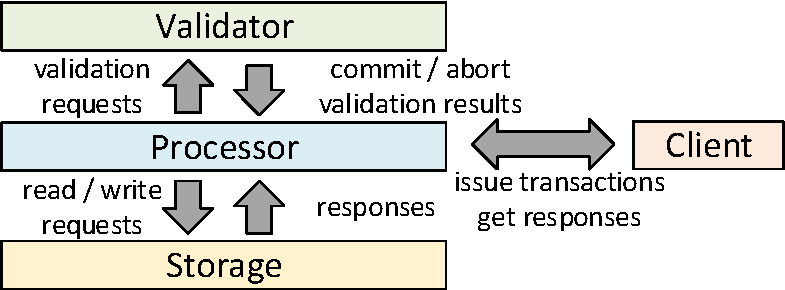
\includegraphics[width=0.9\columnwidth]{figures/arch.pdf}
 \vspace{-.5em}
 \caption{OCC system architecture}
 \vspace{-1em}
 \label{fig:occ_arch}
\end{figure}


% contribution
{\bf Contributions of this Paper.}
In this paper, we explore in-depth the benefits of transaction batching and operation reordering in OCC with backward validation, with a focus on storage and validator batching. Our system design is best suited for integration with an in-memory versioned key-value store, as we require the ability to customize the validation logic. Our previous work on the Centiman system\cite{ding2015centiman} proposed a loosely coupled architecture for OCC on top of key-value stores. The system we present here follows Centiman's architecture and enhances its design with batching and reordering.

% contribution 1: system design
Our first contribution is an enhanced OCC system architecture that utilizes batching and reordering at the storage and the validator levels. We analyze the reasons for conflicts and aborts at each stage of a transaction's life cycle, and develop techniques to reduce these aborts through batching.
% integration of our architecture into a realistic system.


% contribution 2: validator reordering algorithms
Our second contribution is an optimal algorithm for storage reordering and
approximate algorithms for validator reordering. We show that finding the
optimal transaction ordering within a validator batch is NP-hard. We then describe
two classes of greedy algorithms that balance abort rates and reordering overheads. These algorithms produce transaction orderings
that are close to the optimal solution, and are sufficiently fast for
practical use. We also extend these algorithms to weighted versions that can incorporate features such as transaction priorities.\eat{ Thus our second contribution actually enables storage and validator batching in a real system.}


\eat{
As mentioned before, the overhead of validator reordering increases transaction latency. Thus, even as validator reordering reduces the number of conflicts, it may hurt the end-to-end throughput of the system. Our two classes of greedy algorithms explore this trade-off. Additionally, we extend our algorithms to weighted versions that can incorporate features such as transaction priorities.
}

% contribution 3: parallel validation
Our third contribution is a design that reduces the amortized overhead of validation through parallelism. The parallelization is achieved with a four-stage pipeline, where the stages are batch preparation, transaction reordering, transaction validation, and cache update. Each of these stages can be further parallelized to allow concurrent processing. 

% contribution 4: experiment
Our final contribution is a detailed experimental study of the impact of storage and validator batching in a prototype system. Our results show that batching and reordering always increases transaction throughput and, surprisingly, also reduces transaction latency, especially the tail latency. This is because batching and reordering reduces the chance of conflicts and the number of transaction restarts, thus improving the end-to-end transaction latency. For workloads with high data contention, batching and reordering can improve the throughput by up to a factor of 3.1x and can reduce the average transaction latency by up to 68\% for both a micro benchmark and the Small Bank Benchmark~\cite{alomari2008icde}.

%\eat{
% paper organization
The remainder of the paper is organized as follows. In Section~\ref{sec:background}  we review OCC with backward validation. In Section~\ref{sec:overview} we discuss challenges, opportunities and techniques for storage and validator batching. In Section~\ref{sec:validator_reordering}, we introduce our algorithms for intra-batch transaction reordering at the validator. In Section~\ref{sec:experiments}, we present an extensive experimental study of batching in our system. We discuss related work in Section~\ref{sec:relwork} and conclude in Section~\ref{sec:conclusion}.
%}

